\documentclass[12pt]{article}
\usepackage[english]{babel}
\usepackage{natbib}
\usepackage{url}
\usepackage[utf8x]{inputenc}
\usepackage{amsmath}
\usepackage{graphicx}
\graphicspath{{image/}}
\usepackage{parskip}
\usepackage{fancyhdr}
\usepackage{vmargin}
\usepackage{url}
\usepackage{listings}
\usepackage{color} %red, green, blue, yellow, cyan, magenta, black, white
\definecolor{mygreen}{RGB}{28,172,0} % color values Red, Green, Blue
\definecolor{mylilas}{RGB}{170,55,241}



\setmarginsrb{3 cm}{2.5 cm}{3 cm}{2.5 cm}{1 cm}{1.5 cm}{1 cm}{1.5 cm}

\title{Development of LQ Tracker for Inverted Pendulum}								% Title
\author{Mrinmoy Sarkar}								% Author
\date{29 Apr 2015}											% Date

\makeatletter
\let\thetitle\@title
\let\theauthor\@author
\let\thedate\@date
\makeatother

\pagestyle{fancy}
\fancyhf{}
\rhead{\theauthor}
\lhead{\thetitle}
\cfoot{\thepage}

\begin{document}



\lstset{language=Matlab,%
	%basicstyle=\color{red},
	breaklines=true,%
	morekeywords={matlab2tikz},
	keywordstyle=\color{blue},%
	morekeywords=[2]{1}, keywordstyle=[2]{\color{black}},
	identifierstyle=\color{black},%
	stringstyle=\color{mylilas},
	commentstyle=\color{mygreen},%
	showstringspaces=false,%without this there will be a symbol in the places where there is a space
	numbers=left,%
	numberstyle={\tiny \color{black}},% size of the numbers
	numbersep=9pt, % this defines how far the numbers are from the text
	emph=[1]{for,end,break},emphstyle=[1]\color{red}, %some words to emphasise
	%emph=[2]{word1,word2}, emphstyle=[2]{style},    
}


%%%%%%%%%%%%%%%%%%%%%%%%%%%%%%%%%%%%%%%%%%%%%%%%%%%%%%%%%%%%%%%%%%%%%%%%%%%%%%%%%%%%%%%%%

\begin{titlepage}
	\centering
    \vspace*{0.5 cm}
    
\includegraphics[scale = 0.75]{logo.jpg}\\[1.0 cm]	% University Logo
    \textsc{\LARGE North Carolina A\&T State University}\\[2.0 cm]	% University Name
	\textsc{\Large Final project For ECEN-865 Optimal Control Theory}\\[0.5 cm]				% Course Code
	\rule{\linewidth}{0.2 mm} \\[0.4 cm]
	{ \huge \bfseries \thetitle}\\
	\rule{\linewidth}{0.2 mm} \\[1.5 cm]
	
	\begin{minipage}{0.4\textwidth}
		\begin{flushleft} \large
			\emph{Submitted To:}\\
			Dr. Ali Karimoddini\\
            Asst. Professor\\
            ECE Department\\
			\end{flushleft}
			\end{minipage}~
			\begin{minipage}{0.4\textwidth}
            
			\begin{flushright} \large
			\emph{Submitted By :} \\
			Mrinmoy Sarkar\\
            950363260\\
            PhD\\
            msarkar@aggies.ncat.edu\\
            Spring-2018\\
            
		\end{flushright}
        
	\end{minipage}\\[2 cm]
	
	
    
    
    
    
	
\end{titlepage}
\section{Abstract}
In this project a linear quadratic(LQ) tracker is developed for a linear time invariant(LTI) system. The selected LTI system is an inverted pendulum which have four states. The vertical angle of the pendulum is controlled using the LQ tracker. The LQ tracker is developed in MATLAB programming environment and simulated with different reference signal.The controller gain is adjusted in such a way that the overall absolute error between the reference signal and the output signal is less than 0.1. In LQ tracker design the trade off between the input energy and tracking error is shown.
\newpage

%%%%%%%%%%%%%%%%%%%%%%%%%%%%%%%%%%%%%%%%%%%%%%%%%%%%%%%%%%%%%%%%%%%%%%%%%%%%%%%%%%%%%%%%%

\tableofcontents
\pagebreak

%%%%%%%%%%%%%%%%%%%%%%%%%%%%%%%%%%%%%%%%%%%%%%%%%%%%%%%%%%%%%%%%%%%%%%%%%%%%%%%%%%%%%%%%%


\section{Introduction}
The linear quadratic tracker is a very efficient tracker in the context of gain margin and phase margin. The LQ tracker has infinite gain margin and at least $ 60^\circ $ phase margin. So, the tracker is quite robust for stability of the system. In this project a LQ tracker is developed for an inverted pendulum. In the design step, first the mathematical model of the system is developed then the state space representation is formulated with the developed model. In next step, a cost function is defined for the tracking problem and then using the calculus of variation the cost function is minimized. After this formulation, we get two differential riccati equation(DRE) which is solved using Runge–Kutta method. At last the system is simulated with two different reference signal(step and sinusoidal). The following sections are organized as section \ref{System model of inverted pendulum and State space representation}: System model of inverted pendulum and State space representation, section \ref{LQ tracker formulation}: LQ tracker formulation, section \ref{Simulation}: Simulation, section \ref{Conclusion}: Conclusion.
\newpage
\section{System model of inverted pendulum and State space representation \cite{ipendulam}}
 \label{System model of inverted pendulum and State space representation}
The cart with an inverted pendulum, shown in figure \ref{fig:cart}, is "bumped" with an impulse force, F. Determine the dynamic equations of motion for the system, and linearize about the pendulum's angle, $\theta = \pi$ (in other words, assume that pendulum does not move more than a few degrees away from the vertical, chosen to be at an angle of $\pi$).

\begin{figure}[h]
	\centering
	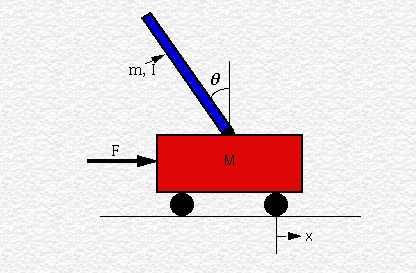
\includegraphics{cart.png}
	\caption{An inverted pendulum}
	\label{fig:cart}
\end{figure}

here,\\
M = mass of the cart\\
m = mass of the pendulum\\
b = friction of the cart\\
I = inertia of the pendulum\\
L = length of the pendulum's center of mass\\
F = impulse force applied to cart
\subsection{Force analysis and system equations}
In figure \ref{fig:freebody} the free body diagram of the system is shown.
\begin{figure}[h]
	\centering
	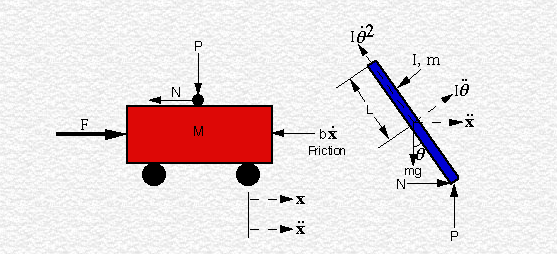
\includegraphics{freebody.png}
	\caption{Free body diagrams of the system}
	\label{fig:freebody}
\end{figure}

Summing the forces in the Free Body Diagram of the cart in the horizontal direction, we get the following equation of motion:
\begin{equation}
M\ddot{X} + b\dot{X} + N = F
\end{equation}
Summing the forces in the Free Body Diagram of the pendulum in the horizontal direction, we get an equation for N:
\begin{equation}
N = m\ddot{X} + mL\ddot{\theta}cos\theta -mL\dot{\theta}^2sin\theta
\end{equation}
If we substitute this equation into the first equation, we get the first equation of motion for this system:

\begin{equation}
(M+m)\ddot{X}+b\dot{x}+mL\ddot{\theta}cos\theta-mL\dot{\theta}^2sin\theta=F
\end{equation}



To get the second equation of motion, sum the forces perpendicular to the pendulum. Solving the system along this axis ends up saving you a lot of algebra. You should get the following equation:
\begin{equation}
Psin\theta+Ncos\theta-mgsin\theta=mL\ddot{\theta}+m\ddot{X}cos\theta
\end{equation}


To get rid of the P and N terms in the equation above, sum the moments around the centroid of the pendulum to get the following equation:
\begin{equation}
-PIsin\theta-NIcos\theta=I\ddot{\theta}
\end{equation}
Combining these last two equations, you get the second dynamic equation:
\begin{equation}
(I+mL^2)\ddot{\theta}+mgLsin\theta=-mL\ddot{X}cos\theta
\end{equation}

 This set of equations should be linearized about $\theta = \pi$. Assume that $\theta = \pi + \phi$ ($\phi$ represents a small angle from the vertical upward direction). Therefore, $cos(\theta) = -1, sin(\theta) = -\phi,$, $\ddot{\theta}^2 = 0$ and $F=u$. After linearization the two equations of motion become:

\begin{equation}
(I+mL^2)\ddot{\phi}-mgL\phi=ml\ddot{X}
\label{eqsys1}
\end{equation}

\begin{equation}
(M+m)\ddot{X}+b\dot{X}-mL\ddot{\phi}=u
\label{eqsys2}
\end{equation}

\subsection{ State space representation of the system}
From equation \ref{eqsys1} and \ref{eqsys2}, we get the state space representation of the system as below:

\begin{equation}
\begin{bmatrix}
\dot{X}\\ \ddot{X}\\ \dot{\phi}\\ \ddot{\phi}
\end{bmatrix}
=
\begin{bmatrix}
0 & 1 & 0 & 0\\
0 & \frac{-(I+ML^2)b}{I(M+m)+MmL^2} & \frac{m^2gL^2}{I(M+m)+MmL^2} & 0\\
0 & 0 & 0 & 1\\
0 & \frac{-mLb}{I(M+m)+MmL^2} & \frac{mgL(M+m)}{I(M+m)+MmL^2} & 0
\end{bmatrix}
\begin{bmatrix}
X\\\dot{X}\\\phi\\\dot{\phi}
\end{bmatrix}
+
\begin{bmatrix}
0\\\frac{I+mL^2}{I(M+m)+MmL^2}\\0\\\frac{mL}{I(M+m)+MmL^2}
\end{bmatrix}
u
\end{equation}

\begin{equation}
y=
\begin{bmatrix}
0&0&1&0
\end{bmatrix}
\begin{bmatrix}
X\\\dot{X}\\\phi\\\dot{\phi}
\end{bmatrix}
\end{equation}

\section{LQ tracker formulation}\label{LQ tracker formulation}
If we have a LTI system like equation \ref{sys1} and \ref{sys2} and if we define the cost function as equation \ref{cfunc}, then the control input of the system would be like equation \ref{soln}. But to get this solution we neet to solve the two differential riccati equation given in equations \ref{riccarti1} and \ref{riccarti2} \cite{lecNote}. The block diagram of the system is shown in figure \ref{fig:blockdig}. The two DREs are solved simultaneously using Runge–Kutta method \cite{rkMethod}. The formula needed to use Runge–Kutta methods is given in equation \ref{eqn:rkmethod}.

\begin{equation}
\dot{X}=AX+Bu
\label{sys1}
\end{equation}
\begin{equation}
y=CX
\label{sys2}
\end{equation}
\textbf{Cost function:}
\begin{equation}
\label{cfunc}
J=\frac{1}{2}(y(t_f)-r(t_f)^TP(t_f)(y(t_f)-r(t_f)+\frac{1}{2}\int_{t_0}^{t_f}[(y-r)^TQ(y-r)+u^TRu]dt
\end{equation}
here, $P\geq0,Q\geq0,R>0$ and all are symmetric.\\


\textbf{Solution:}
\begin{equation}
u=-kX+R^{-1}B^T\nu
\label{soln}
\end{equation}
here, $k(t)=R^{-1}B^TS(t)$

\textbf{DREs:}
\begin{equation}
-\dot{S}=A^TS+SA-SBR^{-1}B^TS+C^TQC;S(t_f)=C^TP(t_f)C
\label{riccarti1}
\end{equation}


\begin{equation}
-\dot{\nu}=(A-Bk)^T\nu+C^TQr;\nu(t_f)=C^TP(t_f)r(t_f)
\label{riccarti2}
\end{equation}
here, $r(t)$ is the reference signal and given over time range $[t_0,t_f]$.\\
\begin{figure}[h]
	\centering
	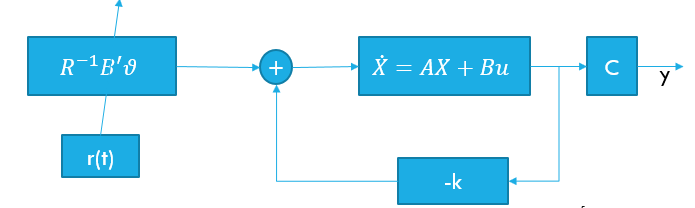
\includegraphics[scale=0.7]{blockdiagram.png}
	\caption{Block diagram of the system with LQ tracker}
	\label{fig:blockdig}
\end{figure}
\newpage

\textbf{Equations for Runge–Kutta method:}

\begin{align}
\label{eqn:rkmethod}
\begin{split}
&\dot{y} = f(t,y) ,
\\
&y(t_0) = y_0 ,
\\
&y_{n+1} = y_n+\frac{dt}{6}(k_1+2k_2+2k_3+k_4),
\\
&t_{n+1}=t_n+dt,
\\
&k_1=f(t_n,y_n),
\\
&k_2=f(t_n+\frac{dt}{2},y_n+dt\frac{k_1}{2}),
\\
&k_3=f(t_n+\frac{dt}{2},y_n+dt\frac{k_2}{2}),
\\
&k_4=f(t_n+dt,y_n+dtk_3).
\end{split}
\end{align}


\section{Simulation}\label{Simulation}
Matlab  programming language is used for the simulation of the system. The parameters of the simulation is given in table \ref{table-para}. Reference tracking signals are shown in figure \ref{fig:step-ref} and \ref{fig:sin-ref}. Corresponding output of the system are shown in figure \ref{fig:step_output} and \ref{fig:sin_output} and the absolute error in tracking are shown in figure \ref{fig:step_error} and \ref{fig:sin_error} respectively.


\begin{table}[h]
	\centering
	\caption{Simulation parameters}
	\label{table-para}
	\begin{tabular}{|l|l|}
		\hline
		Name & Value     \\ \hline
		M    & 0.5 $kg$     \\ \hline
		m    & 0.2 $kg$     \\ \hline
		b    & 0.1       \\ \hline
		I    & 0.006 $kg.m^2$ \\ \hline
		g    & 9.8 $m/s^2$   \\ \hline
		L    & 0.3 $m$      \\ \hline
	\end{tabular}
\end{table}
\newpage
\begin{figure}[h]
	\centering
	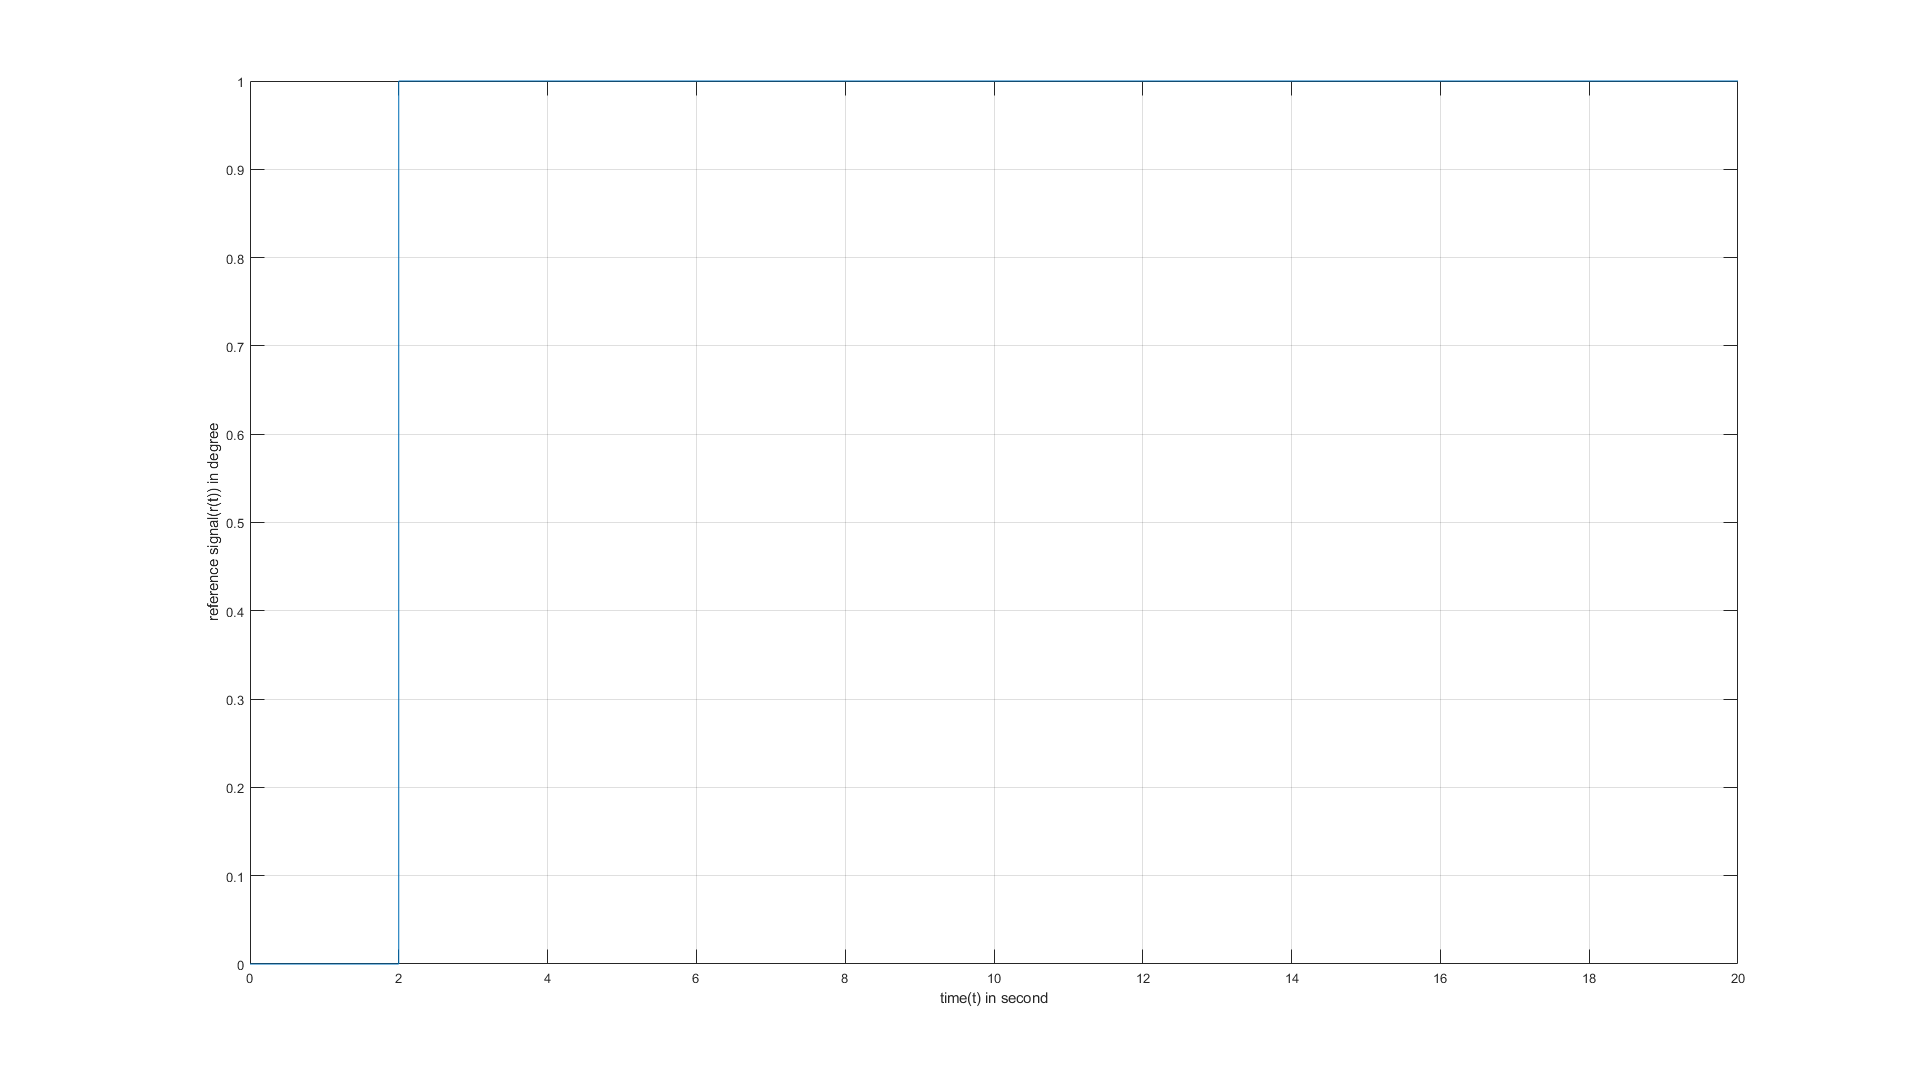
\includegraphics[height=1.8in,width=5.5in]{step_ref.png}
	\caption{Step reference signal}
	\label{fig:step-ref}
\end{figure}
\vspace{2cm}
\begin{figure}[h]
	\centering
	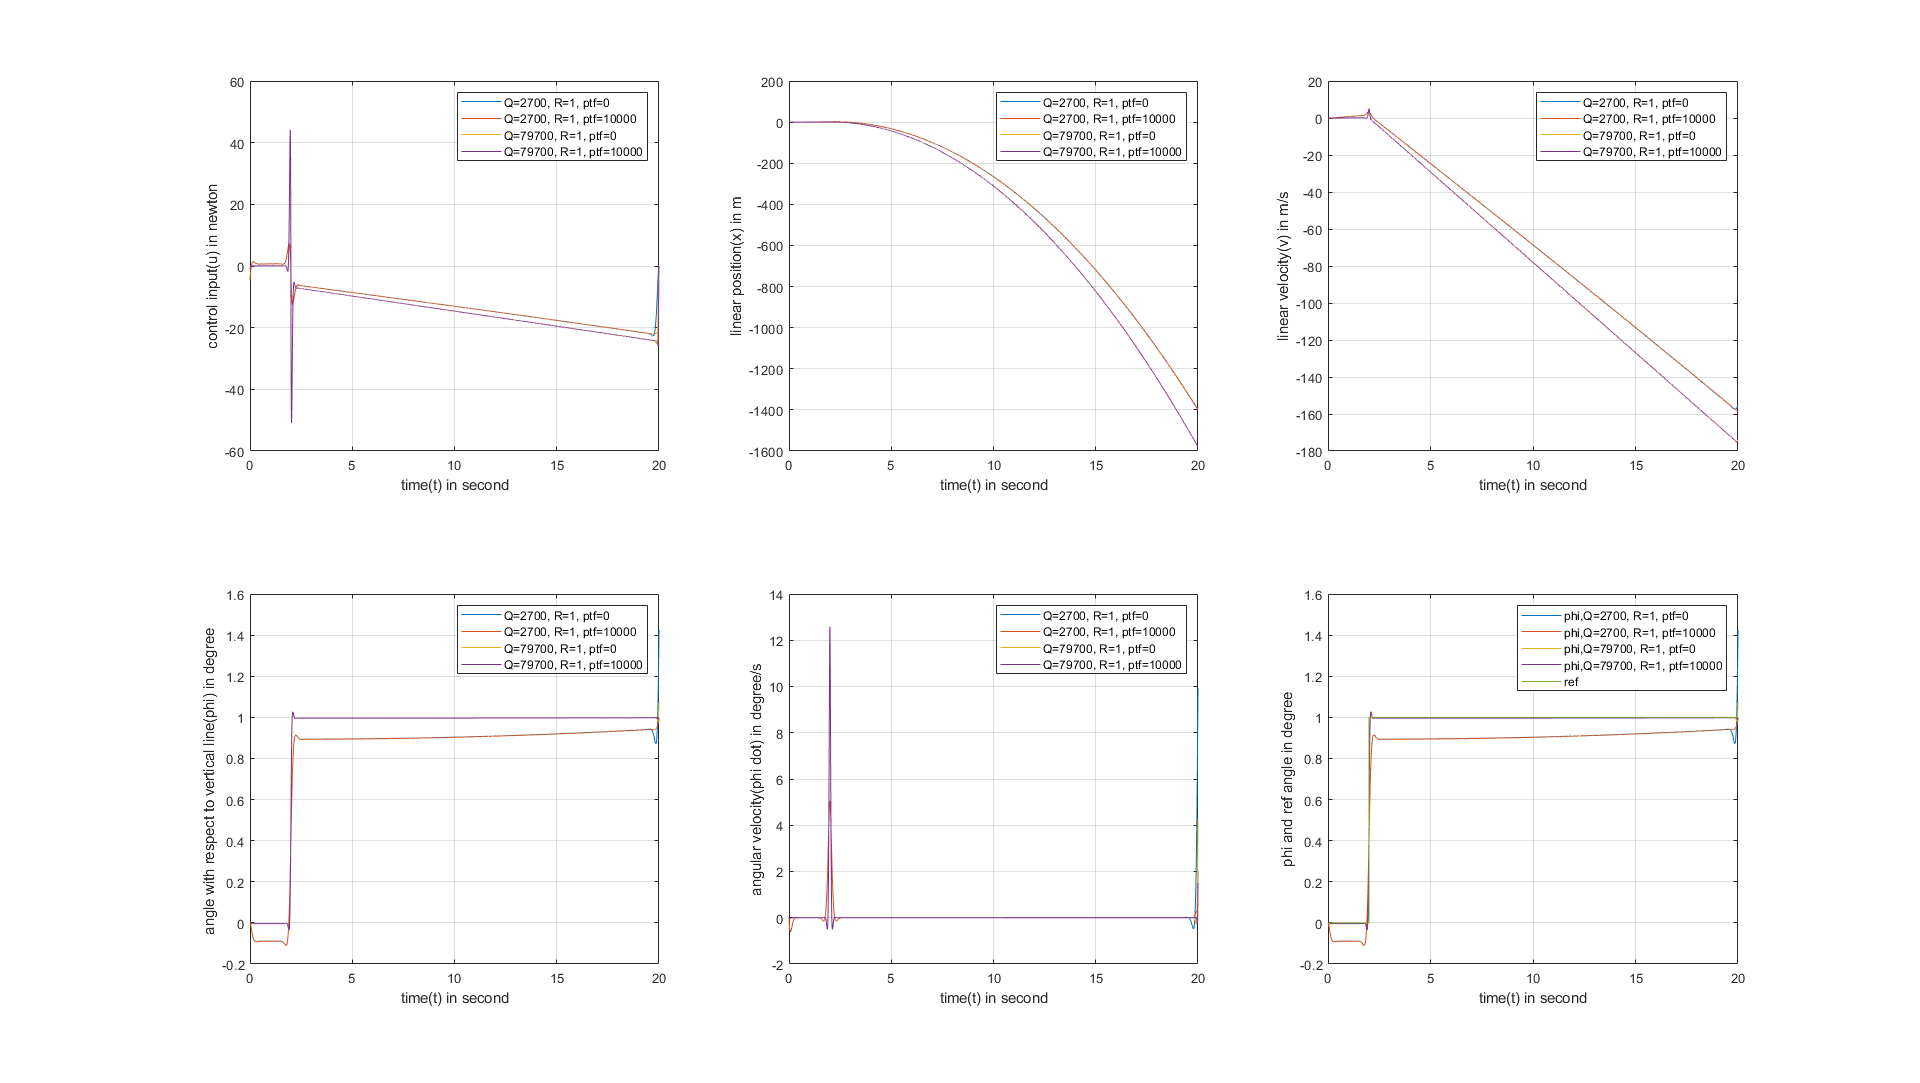
\includegraphics[height=3.4in,width=5.5in]{step_output.png}
	\caption{Output of the system for step reference signal}
	\label{fig:step_output}
\end{figure}
\newpage
\begin{figure}[h]
	\centering
	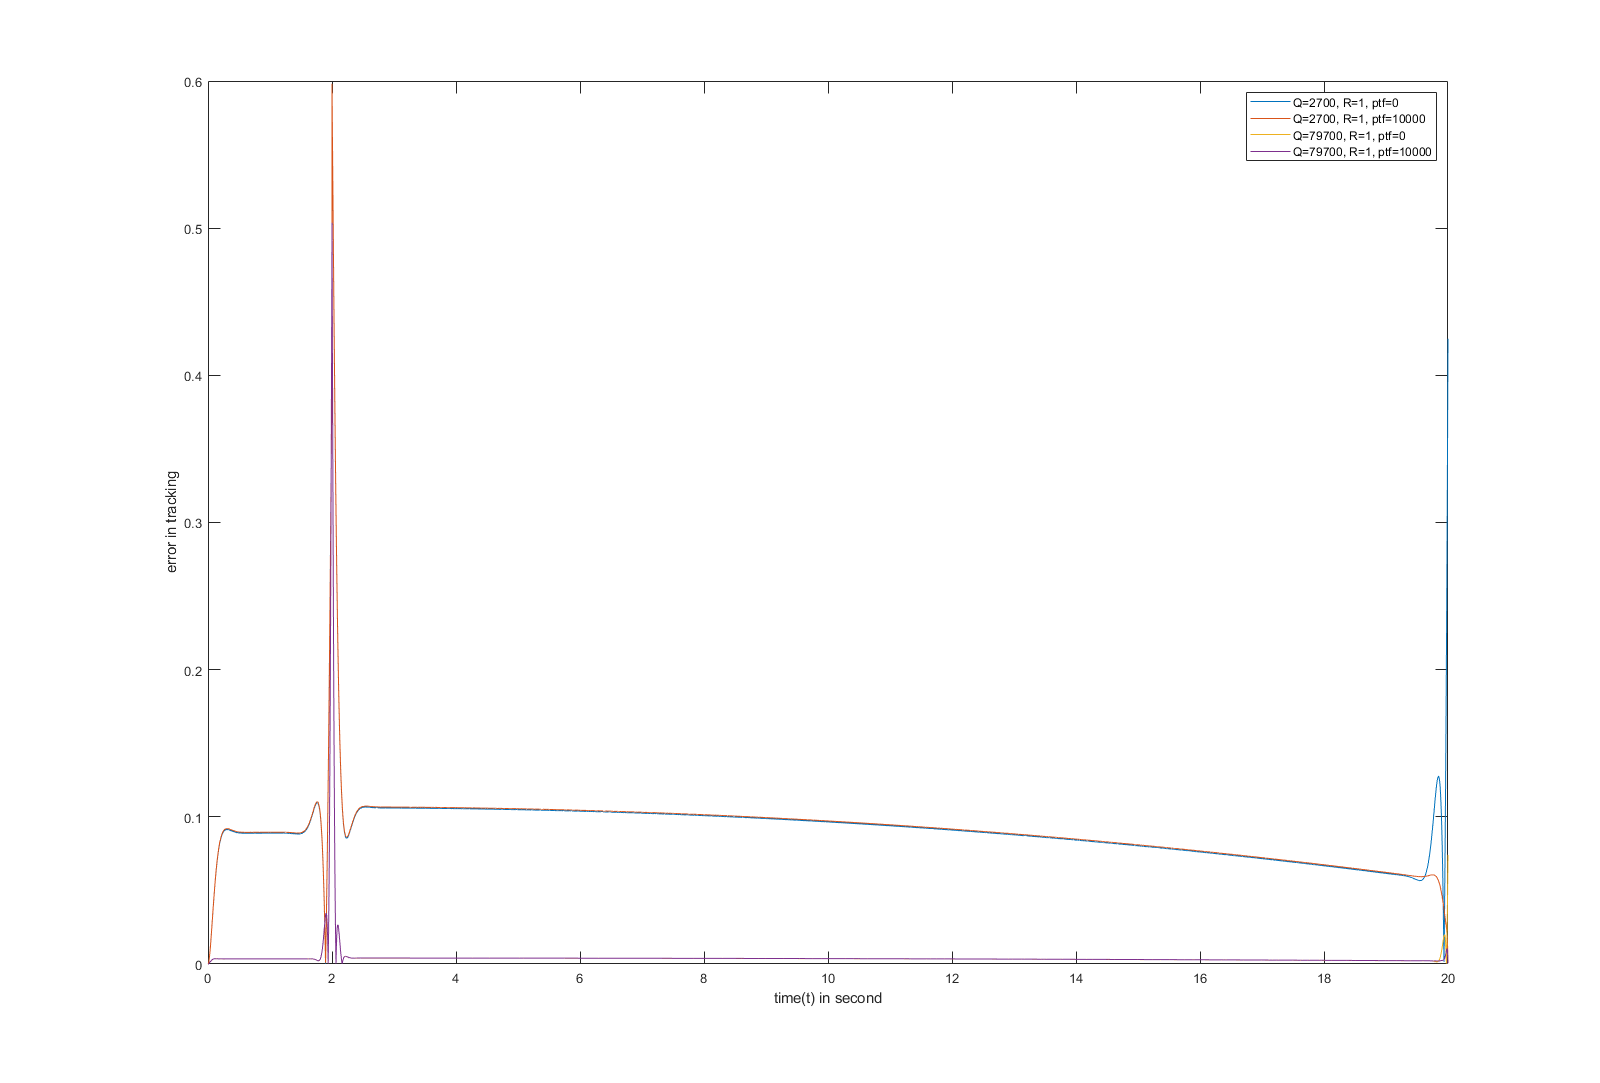
\includegraphics[height=3.3in,width=5.5in]{step_error.png}
	\caption{Absolute error in tracking for step reference signal}
	\label{fig:step_error}
\end{figure}
\vspace{2cm}
\begin{figure}[h]
	\centering
	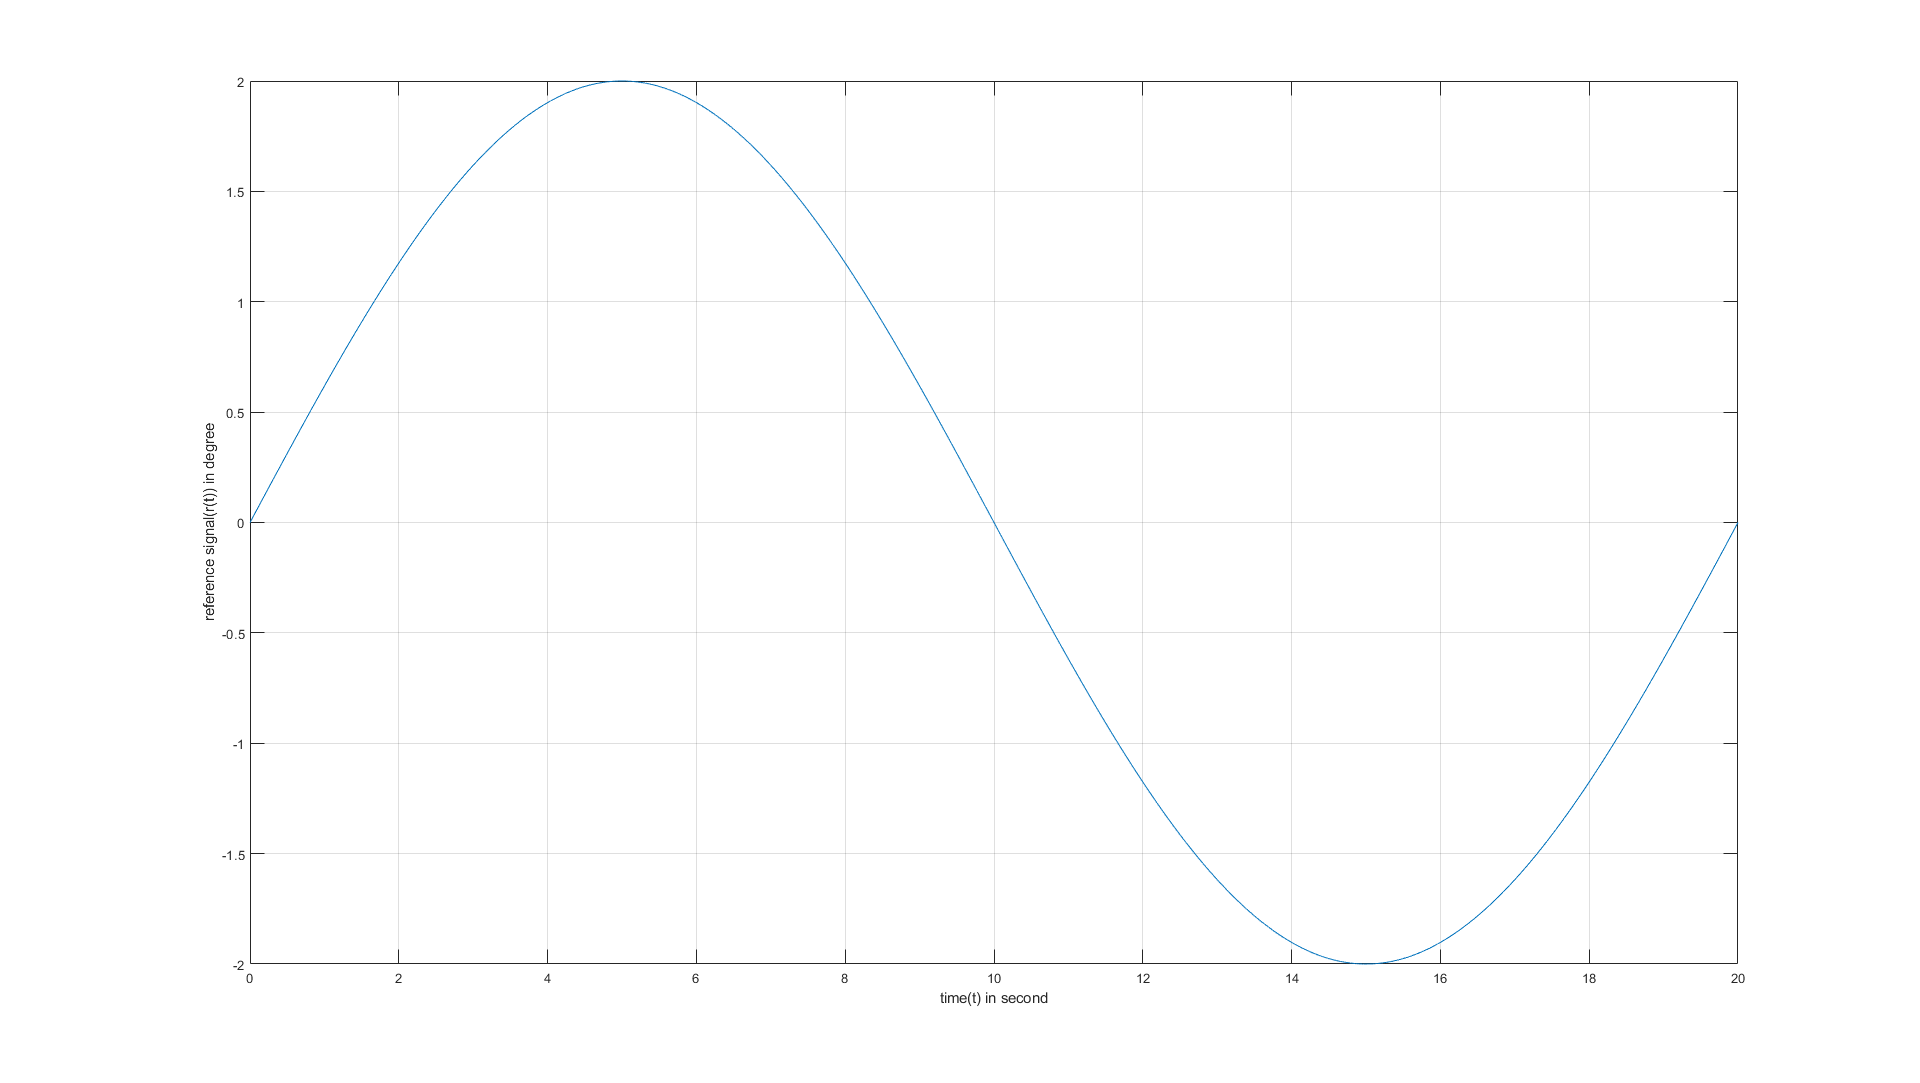
\includegraphics[height=1.8in,width=5.5in]{sin_ref.png}
	\caption{Sine reference signal}
	\label{fig:sin-ref}
\end{figure}
\newpage
\begin{figure}[h]
	\centering
	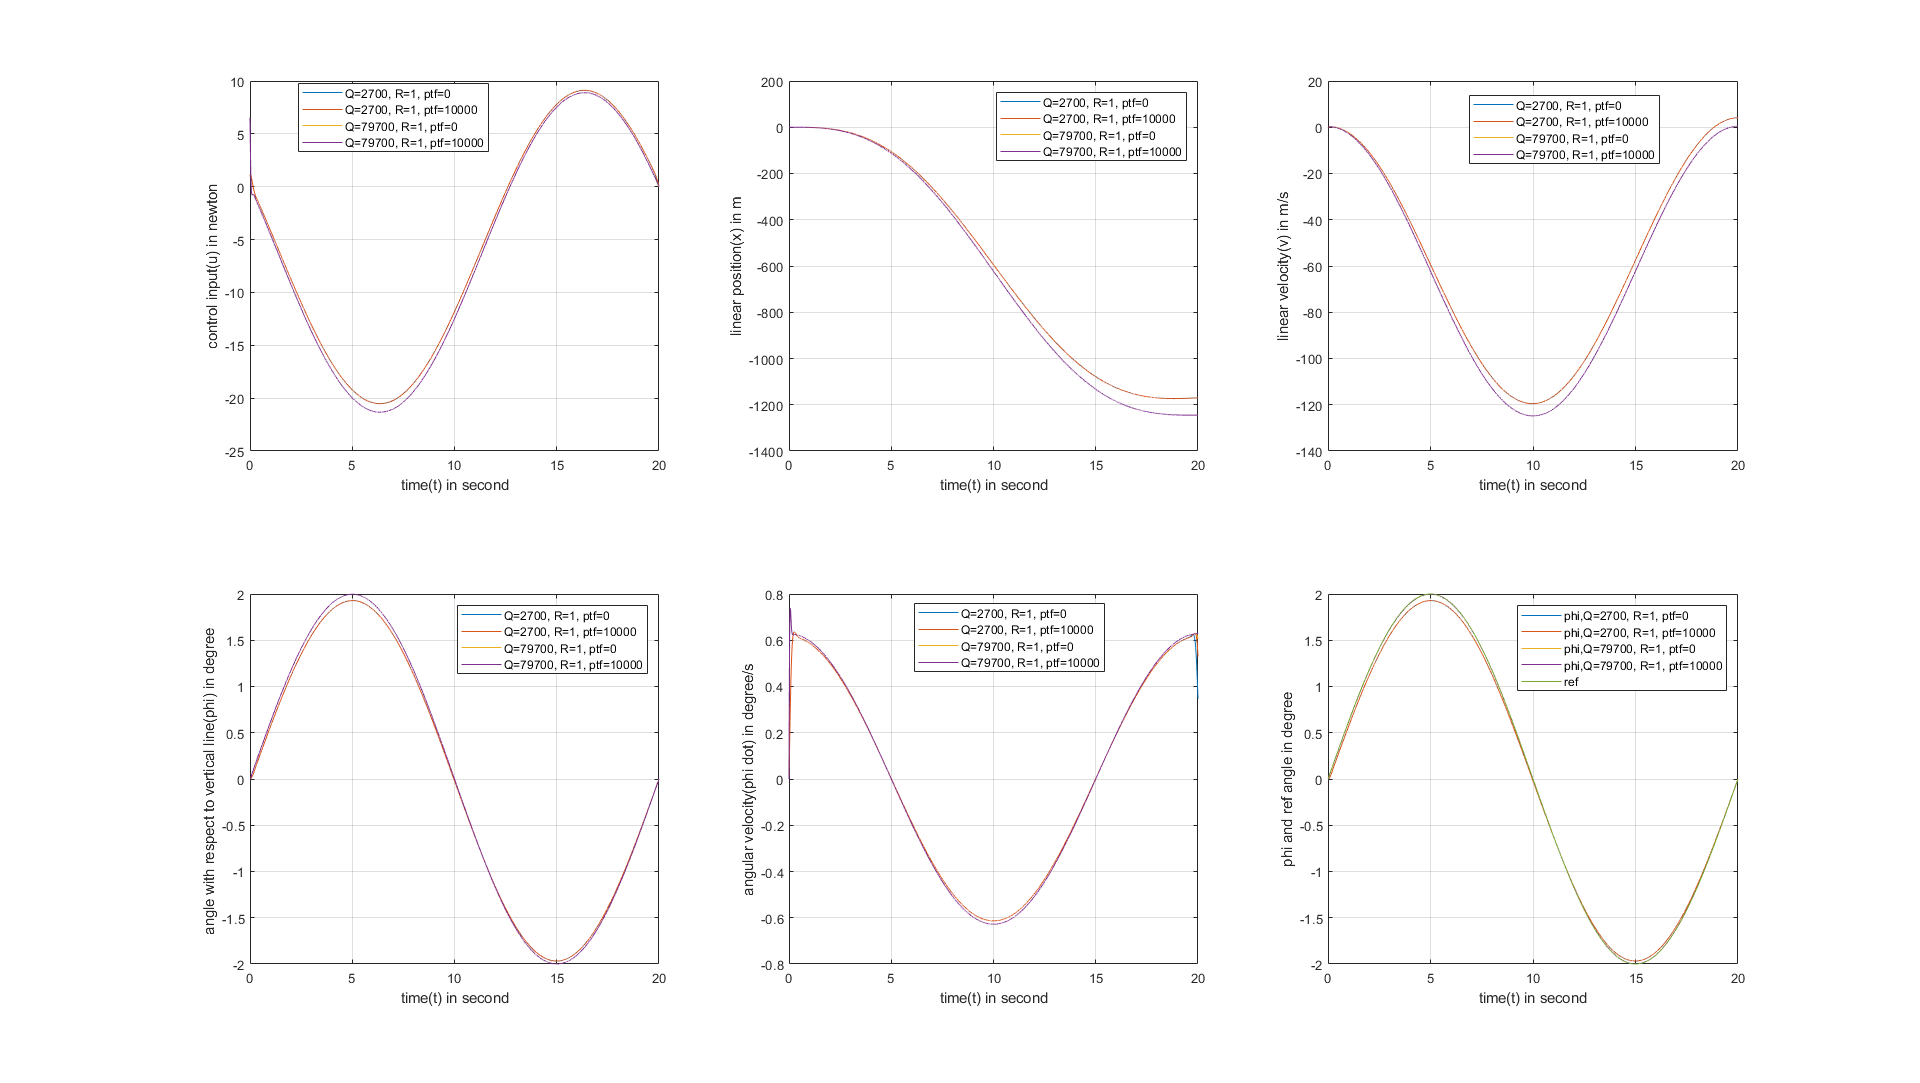
\includegraphics[height=3.4in,width=5.5in]{sin_output.png}
	\caption{Output of the system for sine reference signal}
	\label{fig:sin_output}
\end{figure}
\vspace{2cm}
\begin{figure}[h]
	\centering
	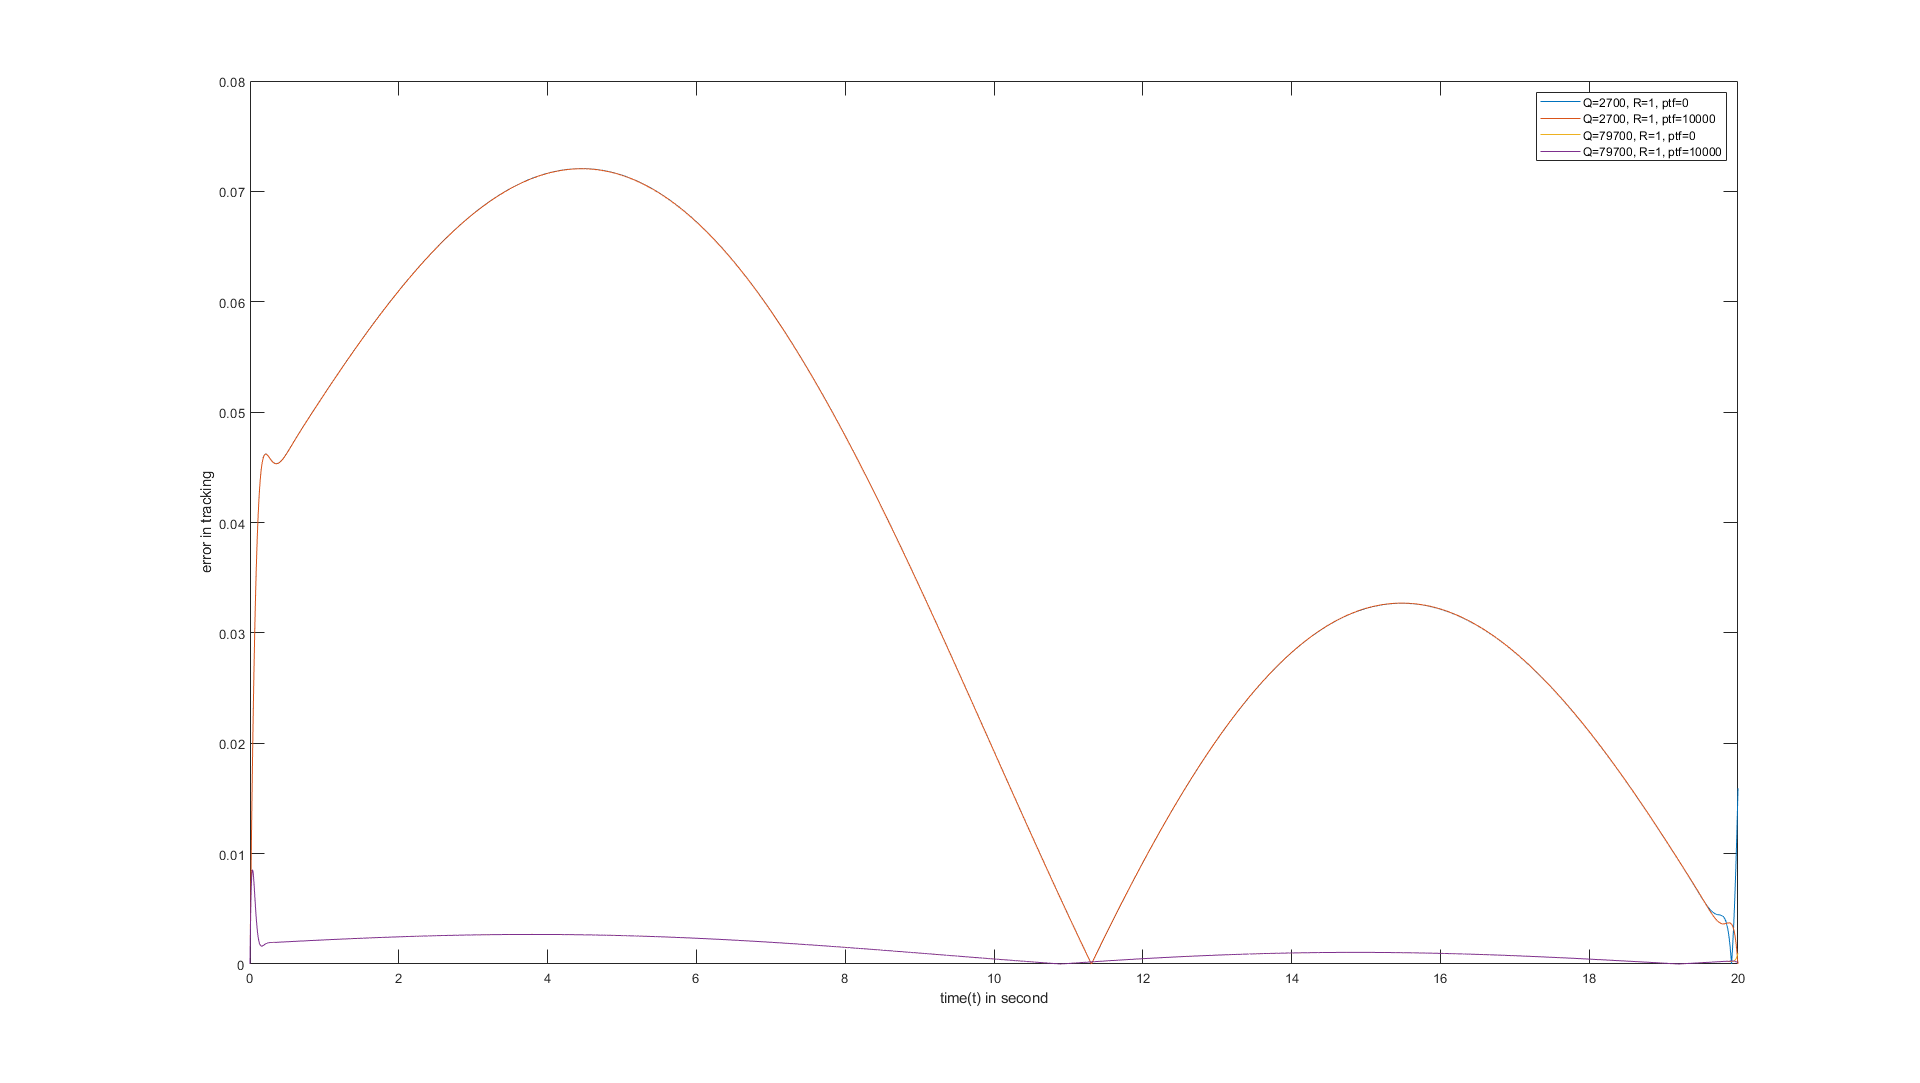
\includegraphics[height=1.8in,width=5.5in]{sin_error.png}
	\caption{Absolute error in tracking for sine reference signal}
	\label{fig:sin_error}
\end{figure}
\newpage

\section{Conclusion}\label{Conclusion}

\begin{enumerate}
	\item In this project LQ tracker is developed and simulated with two reference signal.
	\item The two DRE is solved simultaneously using Runge–Kutta method.
	\item The control input is kept in reasonable value.
	\item The over all absolute error of the tracker is less than 0.1
	
\end{enumerate}

\appendix
\section{\\ \textsc{Matlab} Code}
\lstinputlisting{optiml_tracking.m}
\bibliographystyle{plain}
\bibliography{refs}

\end{document}